\chapter{Plasmonic Stopped Light Lasing}

\section{Introduction} \label{sec:sllIntro}
The speed at which light travels in vacuum is a fundamental property of the
universe and is the upper limit on the speed at which energy can be
transferred.
This speed is outside the scale of normal human experience, and in the context
of nano-optics is considerable at 299.792458 μm/ps.
This high speed does present a problem when storing light-energy, however;
light does not readily slow down.
In the presence of polarising or magnetising media, light will be slowed by a
factor defined as the \emph{refractive index}, which typically is no larger than
about 5, with the largest bulk refractive index known being that of a
metamaterial with an index of 33 \cite{Choi2011}.

The reduction in speed can be improved on by considering the wave nature of
light, and in a chosen frequency interval, modifying the
\emph{dispersion relation} of a wavepacket through resonant phenomena.
This is the field of inquiry of \emph{slow} or \emph{stopped light} (\sl), and
is studied within a broad range of research areas from where the resonant
phenomena can be derived \cite{Khurgin2005}.
These range from
\emph{electromagnetically induced transparency} in cold atom gases
\cite{Hau1999,Liu2001,Lukin2001,Boyd2009}
and in solid state devices
\cite{Ibanescu2004,Yanik2004,Ibanescu2005,Zhang2008,Papasimakis2008},
to \emph{periodic backreflectance} in photonic crystal structures
\cite{Vlasov2005,Krauss2007,Baba2008}
semiconductor quantum wells \cite{Ku2004},
and \emph{Goos-Hänchen shift} \cite{Berman2002} in negative refractive index
metamaterial structures \cite{Tsakmakidis2007,Kirby2011}.
These approaches are not without issues to overcome.
Applications in optical information processing would require integrated
structures operating under ambient conditions, which limits the utility of cold
atom gases in this context.
Photonic crystals rely on periodic structuring, where stopped light resonances
are vulnerable to imperfections and disorder, reducing the speeds to
hundredths of the vacuum velocity but falling short of complete stopping
\cite{Mookherjea2007,Engelen2008}.
Metamaterials, on the other hand, require operation to be on lengthscales where
the meta-atoms are effectively homogenised \cite{Smith2004}, and require
intricate patterning within these scales \cite{Zhang2005,Valentine2008}, though
the chief problem with metal based metamaterials is Drude loss
\cite{Stockman2007,Kinsler2008}.

In this thesis, stopped light is considered in the context of planar
nanoplasmonic structures \cite{Karalis2005}.
Plasmonic stopped light is also robust against disorder, as shown in
Ref.~\cite{Tsakmakidis2014}, but will not be discussed in detail here.
Whereas plasmonic structures are still susceptible to Drude loss faced in the
metamaterial case, this can be compensated for by the inclusion of a gain
material.
Finally, the composition of such plasmonic structures is simple and lends
itself well to experimental realisation.

Stopped light brings about an enhanced density of states \cite{Yao2009} and
allows for the localisation of light coherently over long timescales, which can
enhance nonlinear effects \cite{Franken1961} and interaction with active
components \cite{Lakowicz2004,Fu2011}, making stopped light relevant for
applications in the light harvesting of solar cells
\cite{Aubry2010,Jang2011,Callahan2012}, quantum
information processing \cite{Liu2001}, and optical memories \cite{Zhang2009} as
well as applications in optical communications \cite{Mok2005}.

One of the implications of stopped light, that is perhaps its most interesting,
is \emph{stopped light lasing}.
When designing a laser there are, broadly, two components that must be
considered - gain and feedback.
Gain is the mechanism by which photons (or indeed plasmons) are generated by
stimulated emission.
Here a photon will induce the relaxation of an electron from one state to
another of lower energy, and crucially, emit a second photon that is coherent
with the first.
This process can be repeated, and while the electron population is inverted
(that is there are more electrons in the upper rather state, rather than the
lower), will grow the number of photons in a
coherent state exponentially.
The gain media that are available include semiconductors in bulk
\cite{Kenyon2002}, quantum dots \cite{Plum2009} and wells \cite{Carrere2006},
as well as organic laser dye molecules \cite{Sperber1988}.

Feedback, on the other hand, is the means by which the photons emitted are
coupled back to interact with the same gain medium, such that they may stimulate
further emission.
Most lasers will use a resonant cavity for this purpose, where the cavity modes 
localise electromagnetic energy over a gain medium.
In the field of nanolasing there have been many such examples including
photonic crystal defect modes \cite{Painter1999,Altug2006}, microcavity
resonators
\cite{Iga1988,McCall1992,Vahala2003},
and even the multiple scattering of a “random laser”
\cite{Cao2003,Wiersma2008}.

Stopped light offers an alternative mechanism for feedback than with a cavity.
\sl modes are only confined in one spatial dimension, and not in the other two.
This permits a continuum of planewave solutions, i.e. \sl modes are
propagating waves, rather than standing waves, albeit at zero group velocity.
The lasing mode of a stopped light laser forms dynamically, based on the gain
support for the continuum of modes instead of being predetermined by the
geometry of a cavity.
Here the feedback is provided by a balance of adjacent forward and backward
power flows that form a closed-loop optical vortex which gives rise to the zero
group velocity.

In this chapter, we seek \emph{stopped light structures}, these are
heterogeneous media, whose dispersion relations have at least one zero group
velocity point, i.e. $\Re \dd{\ω}{q} = 0$ for some finite values of the
wavevector $q$.
In such structures, wavepackets of light are pinned and do not drift away
albeit still propagating with a finite phase velocity.
Though to spatially confine light over long timescales, it is not enough
just to have a zero group velocity, one needs to also minimise the dispersion
and material losses.

The energy confinement of stopped light provides the basis for the feedback
mechanism required for lasing to occur.
Nanoplasmonic stopped light lasing is shown to provide a robust mechanism for
the ultrafast excitation of coherent surface plasmon polaritons from simple,
experimentally realisable, subwavelength structures.

\subsection{Organisation of chapter}
This chapter is structured as follows:
In \sec{pvgvd} the dispersion relation of light is explained, introducing
phase, group, and dispersion velocities.
This is followed by a discussion of the differences between a complex frequency
and complex wavevector picture of dispersion in \sec{cwcf}.

The features that make a good stopped light structure, how to find and optimise
structures that possess these, and finally how to excite stopped light modes are
presented in \sec{plasSLS}.
An optimised structure is then analysed in frequency domain, including how
plasmon modes can become undamped with the inclusion of a gain medium in
\sec{fdGain}.

Time domain simulations are performed in \sec{tdSims}.
These are based on a four level system model for the gain (\sec{4lvl}).
\Sec{lasingDynamics} investigates how the lasing mode is onset as gain density
is increased, for a stopped light structure and a non-stopped control
structure.
Then in \sec{lasingMode} the spatial and temporal characteristics of the lasing
mode is examined as the width of the gain medium is reduced, exploring the
confinement and output of the lasing mode.

The results are summarised and the chapter is concluded in \sec{slConc}.

\section{Phase Velocity, Group Velocity, and Dispersion} \label{sec:pvgvd}

\begin{figure}
 \includegraphics{figs/sl/Disprel.pdf}
 \caption[Effect of moments of the dispersion relation]{\label{fig:Disprel}
\textbf{Effect of moments of the dispersion relation.}\small\\
A Gaussian enveloped planewave at $t=0$, \subA, is shown individually under the
effects of the moments of the dispersion relation for $t>0$.
Subfigures are paired to have a negative then positive value of an individual
moment, with all others set to zero.\\
\subB, \subC. phase velocity $\vp$ -
envelope remains constant as phase advances.\\
\subD, \subE. loss $\γ$ -
amplitude of the envelope decreases/increases.\\
\subF, \subG. group velocity $\vg$ -
envelope shifts as phase remains constant.\\
\subH, \subI. group loss $\ug$ -
amplitude of envelope increases as phase wavelength increases/de\-creases.\\
\subJ, \subK. dispersion velocity $\vd$ -
envelope widens and a negative/positive chirp is induced.\\
\subL, \subM. dispersion loss $\ud$ -
envelope widens/narrows with no chirp.
}
\end{figure}

Before entering into a study of particular plasmonic stopped light structures,
we first explore how a wavepacket propagates under a
dispersion relation $\ω(q)$, and how its shape evolves as it does.
This will have implications, as will be shown, for the lateral confinement of
such a wavepacket within a finite area.

Consider a wave propagating in one dimension $x$,
with a well defined wavevector, $q_0$, and a narrow spatial bandwidth,
$\σ_0^{-1}$, which gives it a slowly varying spatial envelope with a width
$\sim\σ_0$,
Then the dispersion relation is well described by its Taylor expansion to second
order about $q=q0$,
\begin{equation}
\ω(q) = \vp q_0 + \vg (q - q_0) + \vd\frac{\σ_0}{2} (q - q_0)^2 + \ldots
\;,
\end{equation}
where the following velocities are introduced\footnote{
If three separate velocities seems a lot, in 1977, S.~C.~Bloch reviews seven
previously identified velocities of light in dispersive media and introduces his
own eighth
\cite{Bloch1977}.
} in place of the usual derivative Taylor coefficients:
\emph{phase velocity}, $\vp = \ω(q_0)/q_0$,
\emph{group velocity}, $\vg = \ω'(q_0)$, and
\emph{dispersion velocity} $\vd = \ω''(q_0)/\σ_0$.

A Gaussian wavepacket following this prescription has the functional form,
\begin{equation} \label{eq:tZeroGauss}
\φ(x) = \exp \left(
-\frac{x^2}{2\σ_0^2} + i q_0 x
\right) + \cc
\end{equation}
at a single instant in time, $t=0$.
In order to calculate the time evolution of the wave packet, the function needs
to be expressed in the Fourier domain, where the dispersion relation applies,
\begin{align}
\tilde{\φ}(q) &= \frac{1}{2\π}\int_{-\infty}^{\infty} \d x \: \φ(x) e^{-i q x}
\\
&= \frac{\σ_0}{\sqrt{2\π}} \exp \left(
-\frac{\σ_0^2(q-q_0)^2}{2}
\right)
\;.
\end{align}
In this basis, the time evolution is simply given by multiplication by the
propagator $e^{-i \ω(q) t}$,
\begin{equation}
\tilde{\φ}(q,t) = \tilde{\φ}(q) e^{-i \ω(q) t}
\;.
\end{equation}
The wavepacket then becomes,
\begin{align}
\tilde{\φ}(q,t)
&= \frac{\σ_0}{\sqrt{2\π}} \exp \left(
-\frac{(\σ_0^2 + i \vd\σ_0 t)(q-q_0)^2}{2}
- i \vg (q - q_0) t
- i \vp q_0 t
\right)
\;,
\end{align}
which when transformed back, yields the form,
\begin{equation}
\φ(x,t) = \sqrt{\frac{1}{1+i \vd t / \σ_0}} \exp \left(
-\frac{(x-\vg t)^2}{2(\σ_0^2 + i \vd\σ_0 t)} + i q_0 x - i \ω_0 t
\right) + \cc
\end{equation}
or,
\begin{align} \label{eq:tdGaussian}
\nonumber
\φ(x,t) &=
\φ_0(t) \exp \left(
-\frac{(x-\vg t)^2}{2\σ(t)^2}
\right)
\exp \left(
i q_0 (x - \vp t )
\right)
\\
&\× \exp \left(
i\frac{(x-\vg t)^2}{2\σ(t)^2}
\frac{\vd t}{\σ_0}
\right)
\\ \nonumber
&+ \cc
\end{align}
with the following definitions made:
$\σ(t)^2 = \σ_0^2 + (\vd t)^2 $, and
$\φ_0(t) = \sqrt\frac{\σ_0^2 - i \σ_0 \vd t}{\σ(t)^2}$.

Examining \eq{tdGaussian} term by term;
the first two exponential terms determine that this is a Gaussian function that
is modulated with a planewave of wavevector $q_0$, as in \eq{tZeroGauss}.
The modulation now has a \emph{phase velocity} $\vp$, and the envelope is
centred on $\vg t$, a point that moves in time with the \emph{group velocity}
$\vg$.
The width of the Gaussian increases over time, as determined by $\σ(t)$, which
increases over time proportionally to the \emph{dispersion velocity} $\vd$
and decreases the peak amplitude of the pulse as it spreads, as determined by
$\φ_0(t)$.
The final term is a complex phase factor that determines the \emph{chirp} of the
wave, which at any instant in time, gives a spatial factor
$\exp(i q_\mathrm{c}^2 x'^2)$ (for $x' = x - \vg t$, and $q_\mathrm{c}$ is a
time-dependant constant), which is a complex phasor with a wavelength that
decreases away from a central point.
Another way to envisage this is, when the dispersion relation has a positive
curvature, the local group velocity $\dd{\ω}{q}(q)$ is higher for larger
wavevectors than for small ones, as such higher wavevector components make
their way to the front of the wavepacket, leaving the low wavevector components
at the back.

The previous analysis has presented the time evolution as though the dispersion
relation were real valued, whereas in general, each of the moments has an
imaginary part, which will be denoted as,
\begin{equation}
\ω(q) = \Re \ω(q)+ i\γ + i\ug (q - q_0) + i\ud\frac{\σ_0}{2} (q - q_0)^2
+ \ldots
\;.
\end{equation}
For even order moments $\γ$ and $\ud$, the loss and dispersion loss, positive
values represent gain whilst negative represent loss. The odd moment $\ug$, the
group loss, is alternatingly gainy or lossy either side of the central
wavevector, with the effect of shifting the central wavevector over time .
The effect of all the moments of the dispersion relation is plotted in
\fig{Disprel}.
%need a better name for group loss.

The resulting expansion of a Gaussian pulse evolution is lengthy, therefore its
explicit expression will be omitted here.
The group loss and dispersion loss terms each contribute to the complex phase of
the wavepacket, though this will not be explored further.
The effect on the amplitude however is to multiply by an exponential factor
and to apply a spatial convolution by an additional broadening term\footnote{
For this second order Taylor expansion model to remain valid, the loss
dispersion, $\ud$ should satisfy, $\ud \le 0$ and $|\ud| \gtrsim |\ug|$.
},
\begin{equation}
\φ(x,t) \→ \exp\left(\γ t - \frac{\ug^2}{2\ud\σ_0} t \right) \times 
\frac{\exp\left( \frac{x^2}{2 \σ_0 \ud t} \right)}{|\σ_0 \ud t|}
\otimes_x
\φ(x,t)
\;.
\end{equation}
These additional terms are present because the imaginary part of the dispersion
relation will change the profile of the wavevector spectral density over time,
\begin{equation}
|\φ(q, t)|^2 \propto e^{2[\Im \ω(q)] t}
\;.
\end{equation}
This is in contrast to the real moments of the dispersion relation, which do not
alter the spectral density.

This section has explained how the dispersion relation affects the
space-time propagation of band-limited electromagnetic radiation.
By engineering the dispersion relation, via choice of materials and structuring,
one may seek to control the pulse propagation itself.
This is to include control over the shape of a pulse, and how it drifts
and disperses, but also the phase relations and chirping.

\section{Complex Wavevector and Complex Frequency} \label{sec:cwcf}
The dispersion relation of the modes of a planar heterostructure, as discussed
in \sec{stratmed}, is determined as the condition required to maintain a
nonzero electromagnetic field within a structure in the absence of an external
driving field.
The solutions are planewaves in a direction of propagation perpendicular to the
stacking of the heterostructure, i.e. $\exp(i q x - i \ω t)$, and the
dispersion relation is the range of allowed $q$ and $\ω$ value pairs.
The dispersion can, of course, be expressed in functional form as either
$q_i(\ω)$ or $\ω_i(q)$, where $i$ is the mode index.
The functions are called the \emph{complex wavevector} (\cwv) and
\emph{complex frequency} (\cfr) representations, respectively.
In general both quantities are complex, but expressing them in functional
form allows for the function argument to be given as a real eigenvalue
parameter.
Both descriptions are equivalent, and describe the same space time dynamics.

Consider a structure with a single mode, with a monotonic dispersion relation.
Its spacetime profile can be expressed in the complex wavevector picture as,
\begin{equation}
  \φ(x,t) = \int_{-\infty}^{\infty} \d\ω \:
  \tilde{\φ}(\ω) e^{i q(\ω) x - i \ω t}
\;,
\end{equation}
which could be interpreted at face value as in integral along the real axis, or
alternatively as a complex contour integral along the path $\ω(s)$,
\begin{equation}
  \φ(x,t) = \int_{-\infty}^{\infty} \d s \:\dd{\ω}{s}
  \tilde{\φ}(\ω(s)) e^{i q(\ω(s)) x - i\ω(s) t}
\;.
\end{equation}
If the path is chosen such that $q(\ω(s)) = s$ for all $s \in \reals$,
then the integral becomes,
\begin{equation}
  \φ(x,t) = \int_{-\infty}^{\infty} \d s \:
  \tilde{\φ}(s) e^{i s x - i\ω(s) t}
\;,
\end{equation}
with $\tilde{\φ}(s) = \tilde{\φ}(\ω(s)) \dd{\ω}{s}$,
and this is exactly the complex frequency representation, as parameterised by a
real wavevector $s$.
The mode's spectral content $\tilde{\φ}(\ω)$ is analytically continued from
the real axis to the curve $\ω(s)$.

Given the equivalence of the two pictures, the utility of each must be
discussed.
The complex frequency picture is parameterised with a real wavevector
eigenvalue;
this means that it is a description suited to having a wavepacket with a known
spatial distribution at one instant in time, and calculating the time evolution,
i.e. having energy stored in a structure and calculating how it dissipates.

The complex wavevector picture on the other hand, is suited to knowing the time
evolution of a wavepacket at a single point in space, and then calculating the
propagation of the wave through space. e.g. calculating propagation in a
fibre-optic cable with a known signal input at one end.

For stopped light, it is the complex frequency representation that is the most
useful.
This can be justified both intuitively and mathematically.
Intuitively, we will want to determine the propagation of a wavepacket
with losses at the zero group velocity point.
It makes little sense to consider the complex wavevector (losses in space)
picture as, by construction, we are considering wavepackets that do not
propagate in space.
Conversely losses in time are indeed a meaningful quantity for a stationary
wavepacket.

Mathematically speaking, for a structure with at least one stopped light point,
i.e. where $\Re \dd{\ω}{q} = 0$ for a finite $q$,
this is just a turning point in an $\ω(q)$ description, whereas in a $q(\ω)$
picture, this is a singular point, and multiple branches of the function must be
considered to capture the behaviour about the point.

In practice, stopped light points don't even manifest themselves in the complex
wavevector solutions \cite{Reza2008,Yao2009}, therefore from here on, the
complex-frequency picture is used to analyse the \sl modes of structures
under consideration.

Though the complex-wavevector picture can not describe stopped light itself, it
will be shown that it is well suited to describing the plasmons that are
emitted as an output channel from stopped light lasing.

\section{Plasmonic Stopped Light Structures} \label{sec:plasSLS}
%Figure showing zgv point and flatness

In order to confine light longitudinally in a waveguide, a wide range of
wavevectors must be supported within a narrow frequency range.
A way of achieving this would be to use a structure that supports two
\emph{zero group velocity} (\zgv) points on the same mode.
A \zgv point defines a turning point in the real part of the
dispersion relation, i.e. $\Re \dd{\ω}{q}(q_0) = 0$.
By definition, having two adjacent \zgv points implies that the
dispersion relation in-between is necessarily monotonic, since no further
turning points can exist within the interval.
It is also guaranteed that a point of zero dispersion, $\Re \ddd{\ω}{q} = 0$,
(see \sec{pvgvd}) exists in the range.

The range of wavevectors between the two \zgv points is referred to as a
\emph{stopped light band}.
The quality of such a band will be determined by two factors,
how narrow the frequency bandwidth is, and how broad the wavevector bandwidth
is.
For a pair of stopped light points \zgv1 and \zgv2, the frequency and wavevector
bandwidths are given as $\Δω = \ω_2 - \ω_1$ and $\Δq = q_2 - q_1$ respectively.
This allows for the definition of the \emph{band velocity} $\vb$,
which is the average group velocity between the \zgv endpoints,
\begin{equation}
\vb = \frac{\ω_2 - \ω_1}{q_2 - q_1} = \frac{\Δω}{\Δq}
\;.
\end{equation}
The wavevector bandwidth determines the minimum width that a light
pulse can be confined to, i.e. $\sim 2\π / \Δq$, whereas the frequency
bandwidth will set the overall flatness of the band, and additionally ensures
the operation of the stopped light device to remain quasi-monochromatic, which
becomes important as the stopped light mode is coupled to inverted emitters in a
narrow frequency band (see \sec{fdGain}).

For this study, we consider structures with materials characteristic of a
\threefive semiconductor, i.e. InGaAsP for dielectric layers, and a
transparent conducting oxide \cite{Naik2013}, such as Indium Tin Oxide (\ito)
for metallic layers.
The dielectric is modelled with a constant permittivity
$\ε = 11.68$.
\textsc{Ito}, which has a plasma resonance in the visible which can be
tuned by doping, allowing for operation in the near infrared (i.e. at
telecoms wavelength [$\λ\approx1550\nm$]). It is modelled by a Drude model with
parameters as given in \tab{4lvlParams} provided by experimental data
\cite{Noginov2011}, with the loss reduced by a factor of 10,
which can be achieved through high fabrication quality and at low
temperatures \cite{Khajavikhan2012}.

\subsection{Mode Hybridisation} \label{sec:hybrid}

\begin{figure}
 \includegraphics{figs/sl/HybridMode.pdf}
 \caption[Hybridisation of modes]{\label{fig:HybridMode}
\textbf{Hybridisation of modes.}\small\\
Dispersion relations, $\Re \ω(q)$, are plotted, with the asymptotic light lines
in vacuum $\ω = c q$, and in dielectric $\ω = c q / \εbg^2$, and
surface plasmon frequencies, ${\ωsp}_0 = \ωp/\sqrt{\εinf+1}$ and ${\ωsp}_1 =
\ωp/\sqrt{\εinf+\εbg}$.
Modes of interest are highlighted in deep green, and \zgv points marked in
orange.
\subA. The \spp mode of a metal-air interface, is hybridised with \subB. the odd
mode of a metal-insulator-metal structure, \subC. forming a
metal-insulator-metal-air structure in order to produce a mode with two zero
group velocity points at finite wavevector.
The modes of the “base structures” are included in the background of \subC.
to show the hybridisation.
}
\end{figure}

The dispersion of plasmonic structures is ultimately determined by how its
layers are composed, i.e. their thickness, material, and relative
ordering.
It is possible to predict, and even control, how the dispersion relation will
look before explicitly calculating it.
Having such a model becomes useful in reducing the search space of optimisation
methods discussed in the next section, since calculating the
dispersion relation consists of solving a transcendental equation, which requires
numerical methods.

The predictive power stems from the spatial profile of the plasmonic
mode having peaks on metal/dielectric interfaces with exponential tails,
\begin{equation}
\φ(z) \propto
\begin{cases}
\exp\left( -\Im\κ_+(q) (z-z_0) \right) & z > z_0 \\
\exp\left( \Im\κ_-(q) (z-z_0) \right) & z < z_0
\end{cases}
\;,
\end{equation}
where $\Im\κ(q) > 0$, and broadly increases with $q$.
For small values of $q$, the tails are broad and the mode overlaps with the rest
of the structure, whereas for large $q$ the mode only sees the interface which
it sits at.
Each metal/dielectric interface hosts a surface plasmon, and at low
wavevectors they will overlap and hybridise, while for high $q$ they will
decouple.

This was shown in Ref.~\cite{Karalis2005} with a metal substrate underneath two
dielectric layers, a high index beneath a low index dielectric.
The dispersion relation initially followed the steeper plasmon dispersion of the
metal/low-index overshooting the lower frequency of the asymptotic
metal/high-index surface plasmon frequency which it would tend to for high
wavevectors.
This produced a \zgv point between the two regimes, that was somewhat tunable
by the thickness of the middle layer.

A similar approach can be used for introducing \emph{two} stopped light points.
The two modes to hybridise are that of a \emph{metal-insulator-metal}
(\mim) system \cite{Economou1969}, and a \emph{metal-air} (\ma) plasmon.
The structures and dispersion relations are plotted in \fig{HybridMode}.
The \mim system has two modes, even and odd;
the odd mode (in the $z$ component of the $\E$-field) contains two \zgv points
itself, the first one is at zero wavevector and is not useful being inside the
light cone, the second one is at a high wavevector near where the even and odd
modes become degenerate, and is preserved.

In the combination structure, that is a \emph{metal-insulator-metal-air} (\mima)
system, the odd mode of the \mim system hybridises with the \ma plasmon,
removing the zero-wavevector \zgv point but introducing a new point in the
overlap.
The second \zgv point can also be perturbed and gets pulled in to a lower
wavevector value, depending of the precise structural configuration.

The positions of the \zgv points can be tuned by adjusting the thicknesses of
each layer, while further fine control can be attained by introducing additional
dielectric layers \cite{Karalis2009a}.

\subsection{Evolutionary Optimisation} \label{sec:SLOptimisation}

\begin{figure}
 \includegraphics{figs/sl/GA.pdf}
 \caption[Evolutionary optimisation of stopped light structures]{
 \label{fig:GA}
\textbf{Evolutionary optimisation of stopped light structures.}\small\\
The dispersion relation, group velocity, and fitness metric of a number of \sl
structures. \subA, \subB, and \subC. are tested against the band velocity
metric.
\subD. and \subE. are examples of structures tested under alternate metrics and
with relaxed conditions on materials and layer thicknesses, i.e. (d) Minimising the
second derivative (dispersion) at a \zgv point, (e) Placing the \zgv point at
$q=1\nm^{-1}$, $\ω = 2\π\c/1550\nm$ for a \emph{leaky mode}.
}
\end{figure}

Any given stopped light structure can be optimised using an evolutionary
algorithm, as detailed in \sec{EA}.
The algorithm is seeded with a structure that already has two stopped light
points in one band, as prescribed in the previous section.
The algorithm then generates a number of similar structures, and for each, the
dispersion relation of the corresponding band is calculated.
The structures are assigned and ordered by a fitness metric, where
structures without two \zgv points are flauchinauchinihilipilificated and
immediately discarded. The remaining structures are then passed through the \ea
routine for mutation, recombination and selection.
For the purpose of identifying \zgv points, only the real part of the group
velocity is required to be zero, this is despite the dispersion relation itself
being complex (see \sec{pvgvd}) as it is the real part that determines the shift
of the mode over time.

In order to quantify the quality of a stopped light structure, a fitness metric
must be defined and calculated.
In general this is a functional of the dispersion relation, $f[\ω(q)]$,
(either over the whole curve, or just between the \zgv points).
In practice though, this can be reduced in complexity, and it suffices to just
consider a function of the bandwidths $f(\Δq, \Δω)$.
The landscape of their possible values needs to be considered and how changes in
both variables makes a more or less desirable structure.

The band velocity on face value would seem to be a suitable parameter, as,
\begin{equation} \label{eq:fitnessfn}
f(\Δq,\Δω) = 1 / |\vb|
\;.
\end{equation}
A subtlety does however arise, in that the second \zgv point can tend towards
an infinite value of $q_2$ for finite $\ω_2$, This will send the band velocity
to zero, but allows for an arbitrarily large frequency bandwidth.
To counteract this, a high wavevector cutoff is introduced at around
$\qc\approx 2\π/10\nm$, which modifies the wavevector bandwidth to
$\Δq' = \max(q_2,\qc) - q_1$ which then enters the metric.

Three candidate \sl structures are contrasted in \fig{GA}.
Each of them representing a \threefive{} / \ito heterostructure, but with
varying layer configurations, each layer optimised to the nearest $10\nm$.
The first is an example of a structure with a single stopped light point, which
would be rejected by this particular configuration of the \ea as it fails to
possess two \zgv points, and hence cannot be assigned a fitness metric.
The second structure possesses two \zgv points and covers a wide range of
wavevectors, hence represents a good candidate with a fitness metric of
$f = 131 / c$.
The third structure is an optimised version of the previous one with a lower
band velocity, giving a fitness of $f = 262 / c$.
Albeit its \zgv points are closer together in $q$, there is a smaller frequency
gap, which results in a band velocity around half of its predecessor.
The gradient of the bands can be seen from the dispersion diagram, the
dispersion in \figSub{GA}{.c} exhibits a much flatter band than in \subB.

Two further structures are presented, these have been optimised by the \ea but
with less strict constraints and with different fitness metrics.
The first seeks to minimise the dispersion, $\pdd{\ω}{q}$ at a \zgv
point, rather than the band velocity.
This effectively brings two \zgv points to coalescence rather than spreading
them out, which doesn't guarantee a wide band.
Here a third \zgv point appears in the vicinity of the first
two, this does not contribute directly to the metric, but does make an overall
stronger \sl structure.
The disadvantage to this approach, is that a \emph{second order} \zgv point is
fragile;
Akin to the repeated root of a quadratic equation, a perturbation of parameters
could lead to either two separate \zgv points, or indeed none at all.
Structures can only be tuned to a degree before fabrication tolerances and
disorder will smear their properties.

The second additional structure is one which considers \emph{leaky modes}, where
the fields in the air layer are exponentially growing, rather than decaying,
and the bound modes appear within the light cone.
Leaky modes optimised by this method were analysed for the \emph{photonic}
structure presented in Ref.~\cite{Pickering2014}.
For the structure in \FigSub{GA}{.e}, the target was to place a \zgv point at
telecoms frequency $\ω = 2 \π \c / 1550\nm$ at a wavevector of $q = 1\μm^{-1}$.
i.e. $f = ((\ω-\ω_0)^2/c^2 + (q-q_0)^2)^{-1}$.
This structure used the material properties of Silicon and Silicon Dioxide in
two dielectric layers, with arbitrarily precise thicknesses.
Whereas this structure will not be considered here, as its modes are photonic
in character, a case which has been treated separately \cite{Pickering2014}, it
serves to illustrate the versatility of the \ea for designing structures.

\begin{figure}
 \includegraphics{figs/sl/Dispersion.pdf}
 \caption[Dispersion relation of a stopped light structure]{
 \label{fig:Dispersion}
\textbf{Dispersion relation of a stopped light structure.}\small\\
\subA. Complex frequency mode dispersion relations - The mode of interest is
highlighted in deep green and its \zgv points marked as orange dots.
Also marked are the light line and surface plasmon frequency, both for the
vacuum and dielectric.
\\
\subB. Group velocity log plot of the mode of interest - Positive group
velocities in green, negative in orange. The point of zero dispersion is marked
in grey.
\\
\subC. Description of the structure and energy density throughout the structure
of a planewave of wavevector $q$ in the bound mode.
\\
\subD. Modal loss, $\Im \ω(q)$, up-to the limiting value of $-\γp/2$.
\\
\subE. Complex wavevector modes $\Re \β(\ω)$ - The first four modes are plotted,
the second mode (orange) is of negative phase velocity.
The complex frequency modes are plotted in the background to show the
correspondence.
\\
\subF. Modal loss, $\Im \β(\ω)$, of corresponding complex wavevector modes.
}
\end{figure}

The optimised \sl structure that is used within the rest of the chapter is
presented in more detail in \fig{Dispersion} with properties in \tab{slprops}.
It is composed of an \ito substrate on the bottom, and a
semiconductor layer sandwiched between an \ito strip on top with layers
optimised to the nearest $10\nm$ The modes of this structure are shown alongside
in \figSub{Dispersion}{.b}, and indeed the bound \TM1 mode hosts two \zgv
points.
As a result it exhibits a very flat band with a band velocity of $\vb =
-c/262$.
The mode profile of the energy density of a planewave in the mode is
also shown in dependence of the wavevector $q$.
Being plasmonic in nature, the field is peaked on the interface between the
metallic and dielectric layers, and for low $q$ values, where the
dispersion follows the light cone, it is primarily located in the air layer,
entering the structure for higher $q$ values.
The field has significant value throughout the profile of the dielectric layer
for wavevectors between around $q \in [0.002,0.025] \nm^{-1}$, i.e. while the
plasmons that sit on either side of the dielectric are coupled.
This enhancement of fields is important for stopped light lasing, as it provides
a large overlap between the field profile and an embedded gain medium.

For completeness, the \cwv modes are also presented in \fig{Dispersion}.
To avoid confusion with the \zgv points of the \cfr modes, the complex
wavevector is labelled $\β$ rather than $q$ as previously.
There are an infinite range of \cwv modes, each with increasing imaginary
component; the first four are listed here.
The modes map to the \cfr set in particular places on the dispersion curve, but
pick up large loss where they diverge.

Having, to a large degree, removed the effects of drift and dispersion from our
system, by choosing one with a wide flat band, we are left with loss as the
mechanism that will hinder energy confinement.
For all wavevectors where the dispersion relation departs from the light line,
the system experiences a loss of around $-2 \Im \ω \approx \γp \approx
11\ps^{-1}$.
This will dissipate any energy within the system on such a timescale.
Naturally, the question arises, whether the loss be compensated for, such as by
replacing the dielectric layer with a semiconductor medium, or by explicitly
adding emitters such as quantum dots or gain molecules.

\subsection{Excitation of Stopped Light Modes}
Once a suitable stopped light structure has been selected, the next step is to
excite the stopped light mode.
The usual methods for coupling to a plasmonic waveguide become unsuitable in the
stopped light case.
Bound modes by definition are not coupled to external radiation modes, which is
to say that light energy cannot be transferred to a bound mode by a beam
of light incident on the surface.
This is also linked to the secondary reason, that there is a mismatch
between the wavevector of incident light and the bound modes of a plasmonic
structure, along the direction of propagation\footnote{
The wavevector component normal to the stack is not conserved, so it suffices to
consider the projection in the propagation direction
}.
Incident light is located exactly on the light cone in
energy-momentum space and has a projection in the propagation direction within
it, whereas plasmonic modes are on a line that sits outside the light cone, and
indeed need not be bounded at all in momentum.

In plasmonic structures, one method of coupling is achieved by adding a
local spatial inhomogeneity, such as a prism, or a grating.
In the case of the prism, light is sent down the prism, within the prism's
shallower light cone ($q \le n\ω/c$), this allows for points where the energy
and momentum of both the incoming beam, and the plasmon mode match
\cite{Otto1968}.
In addition to this condition, the prism must be finite in extent, as the
incoming light is part of the radiation spectrum of the “waveguide with prism”
system that will ultimately by transmitted, reflected, or absorbed.
This mode will mix with both the radiation modes and bound modes of the
“waveguide without prism” system, and will decouple from the prism further down
the waveguide.

A grating, which is a periodic patterning of the waveguide along the propagation
direction, acts in a similar way \cite{Ritchie1968}.
The regular patterning allows for scattering between wavevector modes
that are integer multiples of the grating wavevector, $2π/d$, where $d$ is the
period.
This gives a \emph{momentum kick} to the incident light field, allowing it to
match with the dispersion relation of the bound mode.
Again, the radiation mode of the “waveguide with grating” system then mixes with
the bound and radiation modes of the “waveguide without grating”.

These methods are ineffective with stopped light structures because the bound
mode has a low group velocity such that the incident light is unable to get
sufficiently far away from the grating or prism and instead is outcoupled back
through the radiation modes of the combined structures, instead of travelling
far enough for the system to be described by modes without a grating or prism.

Another scheme for incoupling light to a waveguide is end-fire coupling
\cite{Stegeman1983}.
Here the waveguide is assumed to terminate in a plane perpendicular to the
direction of propagation.
If a light pulse is incident on this terminal plane, its profile can be
decomposed into a mixture of bound modes and radiation modes of the waveguide;
the radiation modes propagate away, leaving the bound modes in the system.
This too is unsuitable for exciting stopped light modes, as zero group velocity
modes will not propagate down the structure, they will not enter and instead be
reflected back.
This method of excitation is equivalent to using the complex wavevector
picture, where the temporal profile of excitation at one point along the axis
(the terminal) is known, but as explained in \sec{cwcf}, \zgv points
are not well described in the complex wavevector picture.

A final way to excite the bound modes of a plasmonic waveguide, that is
compatible with stopped light,
is to have them emitted directly from within the structure.
Here, an emitter would be placed within the \sl structure and these would be
pumped to an excited state, such that when they relax, by spontaneous or
stimulated emission, they are able to emit directly into the bound stopped
light mode.

\section{Frequency Domain Gain in the Small Signal Gain Regime}
\label{sec:fdGain} Adding gain to a structure will alter the bound modes that
are supported.
A material that can spontaneously emit photons will also be available to emit
via stimulated processes, thereby adding gain to the system.
This gain will be dispersive in two senses, firstly different frequencies
experience different amounts of gain, and secondly any change to the imaginary
part of the refractive index (i.e. the material gain) will in turn induce a
change in the real part of the refractive index due to causality and the
Kramers-Kronig relations (\sec{KKrels}).
Designing an active \sl structure requires particular care that the introduction
of a gain medium does not damage the stopped light character of the waveguide.

The induced change in mode structure can be analysed using the same transfer
matrix methods of the previous section with the inclusion of a Lorentz
resonance (\sec{DrudeLorentz}) at a defined emission frequency, $\ωe$, to one of
the dielectric layers.
The Lorentz resonance represents the transitions between the levels of a
two-level system with an energy difference $\ħ\ωe$.
In this picture, there is an occupation density of upper and lower levels,
averaged over space, of single two level emitters.
The strength of the resonance is proportional to the \emph{inversion
density} of the two levels, i.e. how much more the higher level is occupied
than the lower one, $\ΔN = N_2 - N_1$, such that a layer with emitters embedded
may be represented by :
\begin{subequations}\subeq
\begin{align}
\ε &= \εbg + \frac{\ωpe^2}{\ωe^2 - \ω(\ω + i \γe)} \\
\ωpe^2 &= -\ΔN \sqrt{\εbg} \γe \σe c
\;,
\end{align}
\end{subequations}
where
$\εbg$ is the permittivity of the layer hosting the resonance, 
$\σe$ is the emission cross-section,
and $\γe$ is the width of the resonance \cite{Wuestner2010}.
Note that for negative inversion, the emitter becomes an absorber as there is a
higher density of emitters in the lower state.

\begin{figure}
 \includegraphics{figs/sl/FdGain.pdf}
 \caption[Perturbation of dispersion relation and loss with Lorentzian
 gain]{
 \label{fig:FdGain}
 \textbf{Perturbation of dispersion relation and loss with Lorentzian
 gain.}\small\\
 The change of mode shape is plotted as Lorentzian gain is introduced to the
 system. For subfigures on the left, emission is about \zgv1, and on the right
 about \zgv2.
 \subA. and \subB. shows a zoom in of how the dispersion relation changes with
 increasing inversion density, while \subC. and \subD. show the corresponding
 loss/gain of the mode.
}
\end{figure}

The \sl structure as presented in the previous section is modified by replacing
the dielectric layer with a Drude-Lorentz emitter (with a $10\nm$ buffer on
both ends of zero inversion density to simulate quenching by the metal layer).
The emission frequency is set to match either one of the \zgv points, and the
other parameters are set as in \tab{4lvlParams} representing the inclusion of
realistic laser dye molecules \cite{Sperber1988}.
The resulting dispersion and loss relations are shown in \fig{FdGain} for
inversion densities $\ΔN$ varying between $0$ and $N$, with a fixed
emitter density, and excitation about \zgv1 and \zgv2.
The first point of note is that, even on full inversion, the addition of gain
does not significantly change the dispersion, with the maximum shift in
frequency being around $0.6\%$.
The presence of \zgv points is preserved, though they may drift slightly, i.e.
\zgv2 moves slightly right with emission about \zgv1.
There is no change at the frequency that is being excited, this
is because the permittivity change of a Lorentzian is zero at the resonant
frequency.
Adding gain has the side effect of making the structure a slightly better
\sl structure as the band velocity is marginally reduced.

The key change though is in the loss.
As the inversion density increases, the loss decreases for wavevectors where the
dispersion is within the gain width.
Initially the plasmons loss is reduced as the inversion increases, then for
an inversion of around $\ΔN/N \approx 0.4$ some wavevectors become undamped, and
even eventually experience gain, Plasmons sitting in these modes will grow
exponentially in amplitude whilst small enough to remain in the
small signal gain regime.
As \zgv2 is flatter than \zgv1, when the emission is about this point, a wider
range of frequencies fall within the gain width, leading to a larger range of
$q$ values that can become undamped.

\section{Time Domain Simulations} \label{sec:tdSims}
A frequency domain analysis can only bring insight so far when describing
processes such as gain, as it is unable to describe nonlinearities.
When plasmons are emitted, electrons are demoted
from higher energetic states to lower ones.
This depletes the population inversion,
reducing the available gain over time, leading to nonlinear dependence in the
field strength.
In addition there are spatial effects to consider, such as spatial hole
burning; the \tmm has assumed uniformity in the direction of propagation,
whereas the level of inversion can vary both in this direction and
perpendicular to the stacking.
Depending on the mode formed, some regions may host higher field densities which
can deplete the local gain.
Thus a dynamic, spatially resolved, time domain simulation is required to
capture all the aspects of emission into a stopped light mode, and as such, in
this section results from \fdtd simulations are presented.

\subsection{Four-Level System} \label{sec:4lvl}

\begin{figure}
 \includegraphics{figs/sl/4lvl.pdf}
 \caption[Schematic of the four-level system]{\label{fig:4lvl}
\textbf{Schematic of the four-level system.}\small\\
 A four-level system is composed of two two-level systems, $\mathrm{a}$ and
 $\mathrm{e}$, with active transitions (0 ↔ 3) and (1 ↔ 2) respectively,
 which are coupled by nonradiative transition rates
 $\τ_{32}^{-1}$ and $\τ_{10}^{-1}$.
 In this scheme, the emission subsystem permits radiative transitions at an
 energy of $\ħ\ω$ and has a slow nonradiative recombination rate
 $\τ_{21}^{-1}$, while the absorption subsystem is electrically pumped at a
 constant rate $\rp$.
}
\end{figure}

The two level system, presented in the previous section, is good for modelling a
single electronic transition, however its inversion density had been set “by
hand”.
There is no way in which a two level system can reach a state of inversion
by relying solely on the processes of spontaneous emission and absorption (the
best that can be achieved is equal occupation of the levels).
A \emph{four-level system} on the other hand can be constructed such that there
can be a dynamically maintained population inversion between two of its levels,
from where stimulated emission can occur.
The construction contains two two-level systems, labelled $\mathrm{e}$ and
$\mathrm{a}$ for emission and absorption; $\mathrm{e}$ is a system with
energy levels 1 and 2 and energy gap $\ħ\ωe$, in-between $\mathrm{a}$, a
system with energy levels 0 and 3 and greater energy gap $\ħ\ωa$, as depicted
in \fig{4lvl}.
The two upper levels, 2 and 3 are coupled by a fast nonradiative
relaxation channel, with rate $\τ_{32}^{-1}$, as are the two lower levels, 0 and
1 ($\τ_{10}^{-1}$).
This has the effect of rapidly depleting the 1\st and 3\rd level shortly after
they become occupied.
Between the levels of the emission two-level subsystem, there is
additionally a slow nonradiative channel ($\τ_{21}^{-1}$).

The key point of a four-level system is that electrons that are pumped
from levels 0 and 3, will quickly decay to level 2, leading to an inversion
density of level 2 over level 1, which is available for stimulated
emission.
In general this would allow the optical pumping between levels 0 and 3 to
generate inversion between levels 1 and 2.
However in this study, rather than optically pumping,  a constant electrical
pump rate $\rp$ is used.
This is done so that the emitted fields, which are tuned to the stopped light
point take the main focus.

Four-level systems are incorporated into \fdtd using the time-domain
differential equation for the polarisation given in \eq{tdDL},
\begin{equation}
\pdd{\Pe}{t} + \γe\pd{\Pe}{t} + \ωe^2 \Pe = {\ωpe^2} \εf \E
\;,
\end{equation}
%where the dye molecules feel a stronger local electric field
%$\Eloc = \frac{\εbg + 2}{3}\E$ than the macroscopic average.
Here the polarisation has been split off into a part $\Pe$ that is
connected with the radiative resonances, it is added to the total polarisation
when entering into the electric field update equations as discussed in
\sec{fdtd}.
The corresponding level occupation densities update with the auxiliary
equations \cite{Wuestner2010},
\begin{subequations}\subeq
\begin{align}
\pd{N_3}{t} &=
\rp N_0 - \frac{N_3}{\τ_{32}} \\
\pd{N_2}{t} &= \frac{N_3}{\τ_{32}} + 
\frac{1}{\ħ\ωe} \left( \pd{\Pe}{t} + \frac{\γe}{2}\Pe \right)
\cdot \E - \frac{N_2}{\τ_{21}} \\
\pd{N_1}{t} &= \frac{N_2}{\τ_{21}} - 
\frac{1}{\ħ\ωe} \left( \pd{\Pe}{t} + \frac{\γe}{2}\Pe \right)
\cdot \E - \frac{N_1}{\τ_{10}} \\
\pd{N_0}{t} &= \frac{N_1}{\τ_{10}} - 
\rp N_0
\;.
\end{align}
\end{subequations}
\emph{Amplified spontaneous emission} (\ase) can be added to this semiclassical
description by including spatially resolved Langevin noise to the system,
which accounts for the dissipative reservoirs feeding back stochastically
on the system.
The noise couples to the four-level system and induces incoherent transitions,
which then become amplified, allowing for the triggering of the lasing
regime \cite{Pusch2012}.

\subsection{Lasing Dynamics} \label{sec:lasingDynamics}

\begin{figure}
 \includegraphics{figs/sl/FdtdScheme.pdf}
 \caption[Schematic of the \fdtd setup]{\label{fig:FdtdScheme}
\textbf{Schematic of the \fdtd setup.}\small\\
The layered structure described in the frequency domain analysis is truncated to
fit in a simulation domain surrounded by \cpml layers.
The pumped gain region is placed in the horizontal centre of the simulation,
and extends a width $w$; vertically it takes up the height of the \threefive layer
that it is embedded in up-to a $10\nm$ buffer on either side.
}
\end{figure}

In this section, the results of and discussions on \fdtd simulations are
presented.
For computational tractability, the simulations presented here are \twod with
uniformity in the $y$ direction.
The layered geometry of \fig{Dispersion} is recreated in these simulations,
with the top and bottom layers (that were unbounded in the analytic study)
having a height of $500\nm$, and the entire structure having a width of
$12500\nm$.
The simulation domain is surrounded with
\emph{convolutional perfectly matched layers} (\cpml) layers,
which quickly attenuate incident fields without introducing reflection such that
they do not interact with the simulation boundary \cite{Roden2000}.
The dielectric layer has a four-level system embedded in it within a region of
width $w$ that varies per simulation in the range $w \in [200, 1500]\nm$,
and a height that is the same height as the host layer with a $10\nm$ buffer on
either side to simulate quenching by the metal layer.
This is depicted in \fig{FdtdScheme} with further simulation parameters that
match the frequency domain analysis as given in \tab{4lvlParams}.

\begin{figure}
 \includegraphics{figs/sl/LasingOnset.pdf}
 \caption[Lasing onset with increasing gain density]{
 \label{fig:LasingOnset}
\textbf{Lasing onset with increasing gain density.}\small\\
\subA, \subB, \subC. Energy density and mean inversion for
\subA. the stopped light structure with a gain density $N=0.002\nm^{-3}$,
\subB. the stopped light structure with a gain density $N=0.001\nm^{-3}$,
\subC. the control structure with a gain density        $N=0.004\nm^{-3}$.
\\
\subD. Power spectra for
\sl structure at $N=0.002\nm^{-3}$ (deep green),
\sl structure at $N=0.001\nm^{-3}$ ($\×5000$ pale green), and
control structure at $N=0.004\nm^{-3}$ (orange).
\\
\subE. Steady state inversion of \sl (deep green) and control (pale green)
structures with varying gain density.
\\
\subF. Steady state cycle averaged energy density with varying gain density.
}
\end{figure}


The first set of simulations examines the general dynamics of emitting into
a stopped light structure.
For a gain region width of $1500\nm$, two sets of simulations are run;
the first with the stopped light structure as described, and the second with a
control structure where the top metal layer has been reduced in thickness
to $20\nm$ with the effect of removing the stopped light points whilst keeping a
\TM1 mode that is in the same frequency range.
In both cases the gain density is varied in a range of $N \in [0.0005,
0.004]\nm^{-3}$.

Of the simulations, the the \sl structure with gain densities above
$N=0.0015\nm^{-3}$ enters a steady state lasing regime after times that vary
between $0.3\ps$ and $0.6\ps$.
Simulations below this density range did not enter into a lasing regime, whereas
there were bursts of \ase, fields never grew strong enough
to lead to sustained lasing.
The control structure also can also enter the lasing regime, albeit requiring
more than double the gain density at $N=0.0035\nm^{-3}$

\FigSub{LasingOnset}{.a-c} plots the mean inversion and energy density of a
point in the centre of the emitter region.
For the cases in the \sl structure that did enter a lasing regime,
characteristic relaxation oscillations can be seen where inversion initially
builds up and spontaneous emission events are induced.
The fields then are amplified as they stimulate further emission, growing the
field in the mode coherently.
From here the emitted fields start to grow exponentially, and when they are of
sufficient strength will deplete the inversion density.
This reduction of inversion feeds back by decreasing the available gain,
leading to a decrease in field energy as the energy in the field is lost to
dissipative processes in the metal layers.
The decrease in energy density allows for the inversion to rebuild.
This continues in an oscillatory manner with the energy density lagging
behind the inversion by 90°.
The amplitude of the inversion and energy oscillations decrease with each
cycle until a stable steady value for both is reached.
In contrast, the control structure, albeit entering a regime of relaxation
oscillations, is more erratic and the oscillations do not settle to a steady
state.
Instead the oscillations continue with a factor of 4 between the peak energy
density and the trough.

Relaxation oscillations are accompanied by a characteristic decrease of the
width of the power spectrum, from a wide peak in \ase,
to a sharp one in the lasing regime, This observation, which is usually taken
as crucial evidence for lasing in experimental setups, is displayed in
\figSub{LasingOnset}{.d}.

For the \sl structure, the inversion density ($N_2-N_1$) needed for lasing is
$0.00148\nm^{-3}$.
If the total density of gain molecules is less than this, then the system
cannot enter a lasing regime, only able to support occasional bursts of
\ase.
Once the lasing threshold has been passed, the energy density in the mode
increases linearly with the gain density.

%Find more things to say here

\subsection{Lasing Mode} \label{sec:lasingMode}

\begin{figure}
 \includegraphics{figs/sl/EnDensPV.pdf}
 \caption[Energy density and flux of lasing mode]{\label{fig:EnDensPV}
\textbf{Energy flux and density of lasing mode.}\small\\
The lasing mode of a \sl structure with a width $1000\nm$.
\subA. and \subB. show the $x$ and $z$ component of the cycle-averaged
Poynting vector respectively, with positive values in green, and negative in
orange.
Focusing on the bottom right lobe of the flux in \subA, energy flows into
the gain region in the dielectric layers and out of it in the metal layer.
For the same lobe in \subB, energy moves downwards out of the gain region
towards the centre, and upwards into the region at the edge.
The counter-clockwise energy vortex in this corner is mirrored in
the other corners.
\\
The cycle-averaged energy density is plotted in \subC. and inversion in
\subD.
The inversion is the complement of the energy density, being highest in areas
with low energy density, and depleted where the mode sits.
}
\end{figure}

In this section, the lasing modes are investigated for \sl structures where
the width of the gain region varies in the range $w \in [200, 1500]\nm$, using a
fixed gain density of $N=0.002\nm^{-3}$.

The spatially resolved, cycle averaged Poynting vector, energy density, and
inversion are plotted in \fig{EnDensPV} for a structure with width $1000\nm$.
The energy is concentrated on metal-dielectric interfaces, strongest on the
lower interface, and is localised around the gain medium despite there
being no cavity along the horizontal direction.

The Poynting vector shows how energy circulates in the structure.
There are four energy flux vortices, one in each corner of the structure, as
described in the figure caption, these have energy move out of the gain region
into the metal layers and into it in dielectric layers.
Considering the $x$ component of the Poynting flux, (\figSub{EnDensPV}{.a}),
the forward and backward flows are in exact balance.
The balanced counter-propagation of energy in the negative-permittivity (metal)
layers against the dielectric layer.
This is the basis of feedback in the system.

The inversion is shown in \figSub{EnDensPV}{.d}, there are areas of spatial hole
burning where the energy density is highest.
The spatial modulation seen is explained when considering the field profile and
its formation.

\begin{figure}
 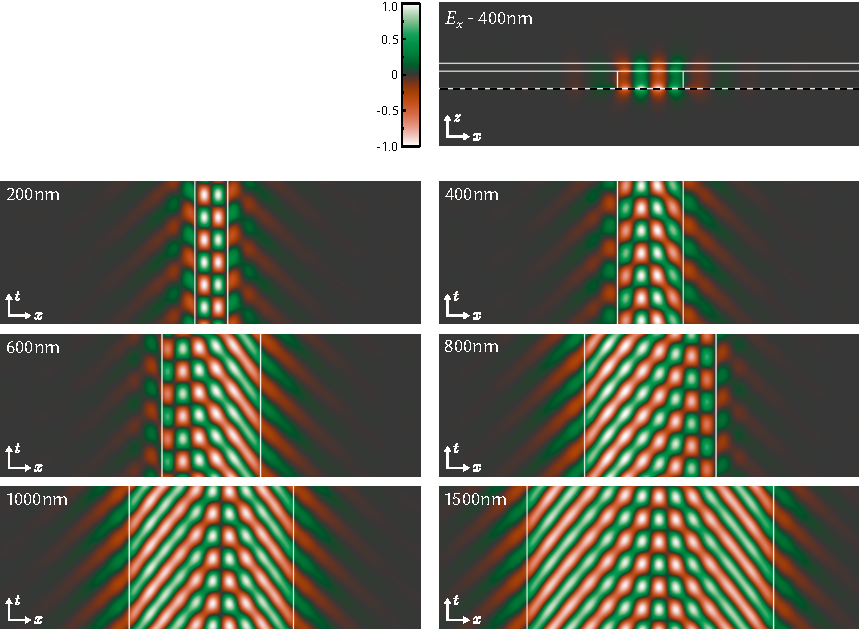
\includegraphics{figs/sl/FieldEvo.pdf}
 \caption[Field evolution in steady state]{\label{fig:FieldEvo}
\textbf{Field evolution in steady state.}\small\\
The $E_x$ field along a line slice at the bottom metal interface is plotted
against time on the vertical axis.
For the $200\nm$ structure, the field inside the gain region is a standing wave.
The other structures have two inward propagating waves which meet at a standing
node.
This node can appear towards the edges, i.e. for $600$ and $800\nm$, or
positioned towards the centre for $1000$ and $1500\nm$.
A stream of plasmons is emitted at either side of the gain region, with a
predominantly negative phase velocity.
}
\end{figure}

It is important to note that the modes that are formed when the structure
enters the lasing regime are a dynamic synthesis of the spectrum of planewave
modes available rather than that of a predefined cavity mode.
The modes that form are propagating waves, with an advancing phase, rather than
purely standing waves, as shown in \fig{FieldEvo}.
It will be shown that this results from modes being centred independently on
finite positive and negative $q$ points, the relative excitation of
each competing with each other, rather than having symmetric excitation at
$q=0$.
This is in contrast even to the stopped light lasing structure considered in
Ref.~\cite{Pickering2014}, which was photonic in nature rather than plasmonic,
and emitted symmetrically about $q=0$ as a standing wave.

In all cases, the modes are inwardly propagating, that is the leftmost half
propagates right and vice versa.
These two halves form a standing wave where they meet, and this node need not be
in the centre of the structure, instead being randomly chosen by the spontaneous
symmetry breaking at the transition from \ase to lasing.
The asymmetry of the mode profile will be discussed later in the chapter.

Lasing is shown to be possible for structures with a gain region width down to
$200\nm$, at which point the steady state inversion rises to around $0.9$.
For this case one observes a standing wave in the gain
interior, i.e. a symmetric excitation of positive and negative $q$ modes.
The confinement of such a structure is at its limit here, with significant
field profile outside the gain region.
For widths smaller than this, there will not be enough gain to pass the lasing
threshold.
This thinnest confinement at $200\nm$ is $12\×$ the free-space wavelength, and
indeed $3.5\×$ the bulk wavelength in the semiconductor layer.

\begin{figure}
 \includegraphics{figs/sl/ComplexQPlasmons.pdf}
 \caption[Complex wavevector plasmons]{\label{fig:ComplexQPlasmons}
\textbf{Complex wavevector plasmons.}\small\\
Power spectra of fields emitted from the right terminal of the gain region
(black dots).
This is fit to the lineshape of the first four \cwv plasmons (green line), i.e.
a Lorentzian function, $|\tilde\φ(q)|^2 = |\sum_i^4\φ_i / (q-\β_i)|^2$.
The amplitudes are varied to fit, but the wavevectors are fixed from the
\cwv plasmon dispersion at the lasing frequency (See \tab{slprops}).
The imaginary part becoming the width in the spectral density.
In each, the negative phase velocity $\β_2$ plasmon is strongest,
with $\β_4$ having a large amplitude for $200\nm$ and $800\nm$ which can be also
seen in the field profiles of \fig{FieldEvo}.
}
\end{figure}

Outside of the gain region, a stream of plasmons is emitted to either side
with a negative phase velocity.
For these plasmons, it makes sense to use a complex-wavevector picture to
describe them, as we have a steady state oscillating source, for which the field
is known at a fixed point in space (the edges of the gain region), for which we
wish to consider the spatial evolution away from this point.

One can analyse the spectral content of the fields, once the system has
entered into a steady state.
Using \emph{discrete Fourier transform} (\fft) methods, the peak frequency
component, $\ωpeak$, of the electric field is identified and isolated.
This returns a spatially resolved, complex valued function $\Etilde(\x,
\ωpeak)$.
Taking a spatial Fourier transform along the waveguide ($x$) axis, allows the
extraction of the spatial power spectrum, which is averaged over $z$ positions
within the gain layer, $I(q) = |\Etilde(q, \ωpeak)|^2$.

The wavevector of the emitted plasmon can be extracted by taking the \fft over
positions outside of the emitting gain region.
\Fig{ComplexQPlasmons} shows the spectrum of fields emitted from the right
terminal, i.e. integrating from the edge of the gain region up to but excluding
the \cpml layer.
These data are fit to the first four analytically determined complex-wavevector
modes (see \fig{Dispersion}) at the lasing frequency.
The wavefunction of such modes is the Fourier transform of a complex decaying
exponential,
\begin{subequations}\subeq
\begin{align}
\φ(x) &= \θ(x)\exp(i \Re \β_i \, x)\exp(-\Im \β_i \, x) \\
\tilde{\φ}(q) &\propto \frac{1}{q-\β_i}
\;,
\end{align}
\end{subequations}
where $\β_i$ is the complex wavevector of the bound mode \spp.
This is summed over each of the first four plasmons, each with a complex
amplitude, then the absolute square of this is compared with the data, i.e.
\begin{equation}
|\φ(q)|^2 = \left| \sum_{i=1}^4 \frac{\φ_i}{q-\β_i} \right|^2
\;.
\end{equation}
The fit allows the amplitude of each resonance to change, but keeps
the wavevectors constant.
Excellent agreement is found, confirming the presence and applicability of the
description of complex-wavevector plasmons.

The negative group velocity plasmon $\β_2$, has the strongest amplitude in all
cases, though the narrow width $\β_1$ plasmon is present too.
In cases where the standing wave node is close to the terminal, i.e. for $w =
200, 400, 800\nm$ there is significant excitation of the short propagation
length $\β_4$ plasmon.

Thus, stopped light lasing can be utilised as a source of coherent plasmons at a
single frequency and discrete wavevector.
Alternatively by adding a grating to the structure away from the gain region,
the plasmons may be outcoupled, converting this into a photonic \sl laser.

\begin{figure}
 \includegraphics{figs/sl/ModeShape.pdf}
 \caption[Power spectrum of lasing modes]{\label{fig:ModeShape}
\textbf{Power spectrum of lasing modes.}\small\\
\subA. Coupling strength $g(q,\ω)$, which is composed of the
emission lineshape (left), the \emph{sinc} function of the gain region (bottom),
and the mode support (overlayed).
The frequency which maximises the the integral of $g$ over wavevector is
\emph{picked} by the system to lase at. \\
\subB. temporal and spatial power spectrum of the lasing mode for model (green
lines) and \fdtd data (black points).
The spatial mode profile is modelled by a modified form of the coupling strength
at the lasing frequency, as given by \eq{lasingShape}.
Results are in excellent agreement with the \fdtd results.
}
\end{figure}

The spatial power spectrum, $I(q)$, can also be taken over the entire domain,
rather than in the interval to the right of the gain region, in order to
capture the profile of the lasing mode.
This function is not symmetric about $q=0$ since it was transformed
from a complex valued function.
Hence it does not follow the usual evenness
properties of the Fourier transform of a real function.
This allows for inspection of how the positive and negative wavevector (and
hence phase velocity) modes are independently excited.
\FigSub{ModeShape}{c} plots the power spectra of lasing modes in the range of
gain widths considered.
It can be seen that in each case, the power spectrum is a bimodal distribution
with peaks about $q \approx \pm 30.7\μm^{-1}$, which is exactly the wavevector
of the second stopped light point.
As one would expect, the width of each peak is inversely proportional to the
gain width chosen, e.g. the smallest gain section at $200\nm$, the width is
around $5\μm^{-1}$.
There is no preferential excitation of the peaks, and
seemingly no correlation between their relative amplitude.
This is because they are two competing modes, one of which will initially
take the lead in growth due to the spontaneous symmetry breaking of amplified
spontaneous emission.
The first mode will dominate the gain, being able to exponentially grow in field
strength.
The second mode may still be allowed to grow but spatially separated from the
first, harvesting areas where the field and gain are less strongly coupled.
This picture is corroborated when viewing the time evolution of the steady state
fields, which show two lobes, inward propagating, with a finite overlap width
where the wave becomes standing, this is depicted in \fig{FieldEvo}.
This is developed further in Ref.~\cite{Wuestner2015}, where it is shown how the
location of the nodes move on longer time scales.

It is possible to predict the spectral content of the lasing mode.
Plasmons are emitted into the frequency which maximises the effective
gain,
\begin{subequations}\subeq
\begin{align}
G(\ω) &=
\int_{-\infty}^{\infty}\d{q} \:
g(q, \ω)
\\
g(q,\ω) &=
\frac{\γL / \π}{(\ω-\ωL)^2 + \γL^2}
\frac{\γpl(q) / \π}{(\ω-\ωpl(q))^2 + \γpl(q)^2}
\sinc^2 \left( \frac{w (q - q_2)}{2} \right)
\,.
\end{align}
\end{subequations}
This expression is the product of three terms;
firstly, there is the emission lineshape of the gain medium,
this is multiplied by the density of states of bound modes that are available to
emit into.
The final part is a geometrical factor, that is the square of the Fourier
transform of a “tophat” function of width $w$, which represents the width of the
gain area.
There can be modulation of the emitted field in the gain region, so the sinc is
allowed to be translated in $q$-space, and will centre itself at the
\zgv2 point $q_2$.
\Fig{ModeShape} shows the frequencies that maximise the effective gain and the
frequency range that was emitted at in the simulations.
This is presented alongside a the coupling strength $g(q,\ω)$ for a $400\nm$
gain section.
This frequency of highest gain can then further be used to predict the mode
shape $I(q)$, up to a factor of the weights of the mode in the $+q$ and $-q$
excitation ($I^+, I^-$),
by a slight modification of $g(q,\ω)$, to include both excitations,
\begin{equation} \label{eq:lasingShape}
I(q) \propto
\frac{\γpl(q)}{(\ω-\ωpl(q))^2 + \γpl(q)^2}
\left(
I^+ \sinc \left( \frac{w (q - q_2)}{2} \right) +
I^- \sinc \left( \frac{w (q + q_2)}{2} \right)
\right)^2
\;,
\end{equation}
which is in excellent agreement with the \fdtd spectra.

\section{Conclusions} \label{sec:slConc}
This chapter has introduced
\emph{plasmonic stopped light lasing}, whereby plasmons are localised by
reducing the group velocity of a wavepacket to zero whilst within a gain medium.
This is in contrast to traditional nanolasing schemes, which localise energy
in a resonant cavity.

In order to explain the concept, topics of dispersion, and the
nuances of the complex-frequency/complex-wavevector pictures have been
discussed.
Frequency domain methods have been employed alongside an evolutionary
optimisation algorithm in order to characterise the properties and quality of a
structure and select for optimal structures within constraints.

An exemplary structure was introduced, composed of realistic
materials, whose properties were studied throughout the rest of the chapter.
Analysis in frequency domain was continued to investigate how, in the small
signal gain regime, a two-level emitting resonator could compensate for the
inherent material losses in metal layers, determining idealised threshold
values of inversion required to free a mode of damping.

Equipped with this analysis, finite difference time domain simulations were made
of the test structure, in order to capture the dynamics of spatial and nonlinear
effects.
The previous frequency domain analysis of the threshold inversion was
corroborated by varying the gain density in each time domain simulation, and it
was found that lasing is indeed possible in this scheme.

The lasing mode was investigated, and a model for predicting its modal content
proposed.
It was found that the feedback provided from stopped light lasing ultimately
derives from a dynamically formed vortex of power flow, with propagation and
counter-propagation balancing between the dielectric and metal layers.
Despite being stopped, the lasing mode carries a finite phase velocity, with an
inward propagating phase modulation that can be detected from the top of the
structure.

As an output of the lasing process, coherent plasmon polaritons (sitting on the
cusp of the complex-wavevector dispersion curve) are emitted from the sides of
the gain region.

This is a new type of subwavelength laser, where the active component is
smaller than a few hundred nanometres, and coherently emits plasmons directly
into a waveguide without relying on external coupling mechanisms.
The dynamic formation of the cavity-free lasing mode is a new physical feature,
the implications of which are open.
It could become the basis for single frequency coherent \spp generation in
quantum plasmonic applications \cite{Jacob2011,Tame2013}, or as the basis of a
quantum fluid such as a photonic Bose-Einstein Condensate \cite{Carusotto2013}.

\begin{table}
 \begin{tabular}{ c | l r l} 
  Symbol	& Parameter 							& Value \\ \hline
  $\εinf$	& Drude high frequency permittivity		& $4.0$		& \\
  $\ωp$		& Drude plasma frequency				& $3130$	& $\ps^{-1}$ \\
  $\γp$		& Drude loss							& $10.7$	& $\ps^{-1}$ \\
  \hline
  $\εbg$	& Background permittivity				& $11.68$	& \\
  $\ωe$		& Emission frequency					& $778$		& $\ps^{-1}$ \\
  $\γe$		& Emission width						& $31.7$	& $\ps^{-1}$ \\
  $\σe$		& Emission cross section		& $\sci{2.12}{-7}$	& $\μm^2$ \\
  $N$		& Carrier density					& $\sci{2}{6}$	& $\μm^{-3}$ \\
  \hline
  $\τ_{10}^{-1}$	& Non-radiative decay rate (0→1)& $10$	& $\ps^{-1}$ \\
  $\τ_{21}^{-1}$ & Non-radiative decay rate (1→2)& $0.002$	& $\ps^{-1}$ \\
  $\τ_{32}^{-1}$	& Non-radiative decay rate (2→3)& $10$	& $\ps^{-1}$ \\
  $\rp$				& Electrical pump rate (0→3)	&  $1$	& $\ps^{-1}$ \\
  \hline
 \end{tabular}
 \caption[Simulation parameters]{\label{tab:4lvlParams}
\textbf{Simulation parameters.}\small\\
Parameters for frequency domain and \fdtd simulations,
divided into:
metal Drude model,
emitter Drude-Lorentz parameters,
\fdtd four-level system parameters.
}
\end{table}

\begin{table}
 \begin{tabular}{ c | l r l} 
  Symbol	& Parameter 						& Value \\ \hline
  $d_1$	& \threefive layer thickness			& $0.110$	& $\μm$ \\
  $d_1$	& \ito layer thickness					& $0.050$	& $\μm$ \\
  \hline
  $q_1$	& \zgv1 wavevector						& $7.41$	& $ \μm^{-1} $ \\
  $\ω_1$	& \zgv1 frequency			& $805 + \i\,4.14$	& $ \ps^{-1} $ \\
  $q_2$	& \zgv2 wavevector						& $30.3$	& $ \μm^{-1} $ \\
  $\ω_2$	& \zgv2 frequency			& $778 + \i\,5.06$	& $ \ps^{-1} $ \\
  \hline
  $\Δq$	& wavevector bandwidth					& $22.9$	& $ \μm^{-1} $ \\
  $\Δω$	& frequency bandwidth					& $26.3$	& $ \ps^{-1} $ \\
  $\vb$	& band velocity							& $1/262$	& $ \c $ \\
  \hline
  $\β_1$	& \cwv mode 1	& $3.94 + \i\,0.131$	& $ \μm^{-1} $ \\
  $\β_2$	& \cwv mode 2	& $-21.3 + \i\,6.71$	& $ \μm^{-1} $ \\
  $\β_3$	& \cwv mode 3	& $51.2 + \i\,6.53$		& $ \μm^{-1} $ \\
  $\β_4$	& \cwv mode 4	& $36.1 + \i\,16.1$		& $ \μm^{-1} $ \\
  			& \cwv frequency			& $778$		& $ \ps^{-1} $ \\
  \hline
 \end{tabular}
 \caption[Properties of optimised \sl structure]{\label{tab:slprops}
\textbf{Properties of optimised \sl structure.}\small\\
Divided into:
Thicknesses of material layers,
coordinates of \zgv points in the dispersion relation,
band metrics,
complex wavevector modes at the \fdtd emission frequency.
}
\end{table}
